
    \documentclass{article}
    \usepackage{amsmath, amssymb}
    \usepackage[T2A]{fontenc} % Cyrillic font encoding
    \usepackage[utf8]{inputenc} % UTF-8 input encoding
    \usepackage{paratype} % PT Serif/Sans fonts with good Cyrillic support
    \usepackage[ukrainian]{babel} % Ukrainian language support
    \usepackage[a4paper, margin=2.5cm]{geometry}
    \usepackage{mathtools}
    \usepackage{xcolor}
    \usepackage{graphicx}
    \usepackage{float}
    \usepackage{enumitem}
    \usepackage{tikz}
    \usetikzlibrary{matrix}
    \usepackage{amsthm}
    \usepackage{booktabs}
    \usepackage{fancyhdr}
    \usepackage{titlesec}
    \usepackage{array}
    \usepackage{longtable}
    \usepackage{siunitx}

    \titleformat{\section}{\Large\bfseries}{\thesection}{1em}{}
    \titleformat{\subsection}{\large\bfseries}{\thesubsection}{1em}{}

    \pagestyle{fancy}
    \fancyhf{}
    \fancyhead[C]{\textbf{Звіт багатофакторної лінійної регресії}}
    \fancyfoot[C]{\thepage}
    \renewcommand{\headrulewidth}{0.4pt}

    \begin{document}

    \begin{center}
    \Large\textbf{Звіт багатофакторної лінійної регресії}
    \end{center}

    \vspace{1cm}

    \textbf{Дата:} \today

    \vspace{0.5cm}

    \section{Опис моделі}

    \begin{itemize}
       \item Залежна змінна: \textbf{Performance Index}
       \item Незалежні змінні: \textbf{Hours Studied, Sleep Hours}
       \item Коефіцієнт детермінації $R^2$: \textbf{0.1419}
       \item Середньоквадратична похибка: \textbf{316.6960}
    \end{itemize}

    \vspace{0.5cm}

    \section{Коефіцієнти регресії}

   \renewcommand{\arraystretch}{1.5} % Increase row height by 50%
    \begin{center}
    \begin{tabular}{lccc}
    \toprule
    \textbf{Змінна} & \textbf{Коефіцієнт} & \textbf{P-значення} & \textbf{Значущість (p < 0.05)} \\
     & \textbf{[95\% довірчий інтервал]} & & \\
    \midrule
    Вільний член & 37.8567 & Н/Д & Н/Д \\
     & [36.3148, 39.3985] & & \\
    Hours Studied & 2.7726 & 0.0000e+00 & Так \\
 & [2.6379, 2.9074] & & \\
Sleep Hours & 0.5397 & 2.7660e-07 & Так \\
 & [0.3340, 0.7455] & & \\

    \bottomrule
    \end{tabular}
    \end{center}

    \vspace{1cm}
    
    \begin{figure}[H]
       \centering
       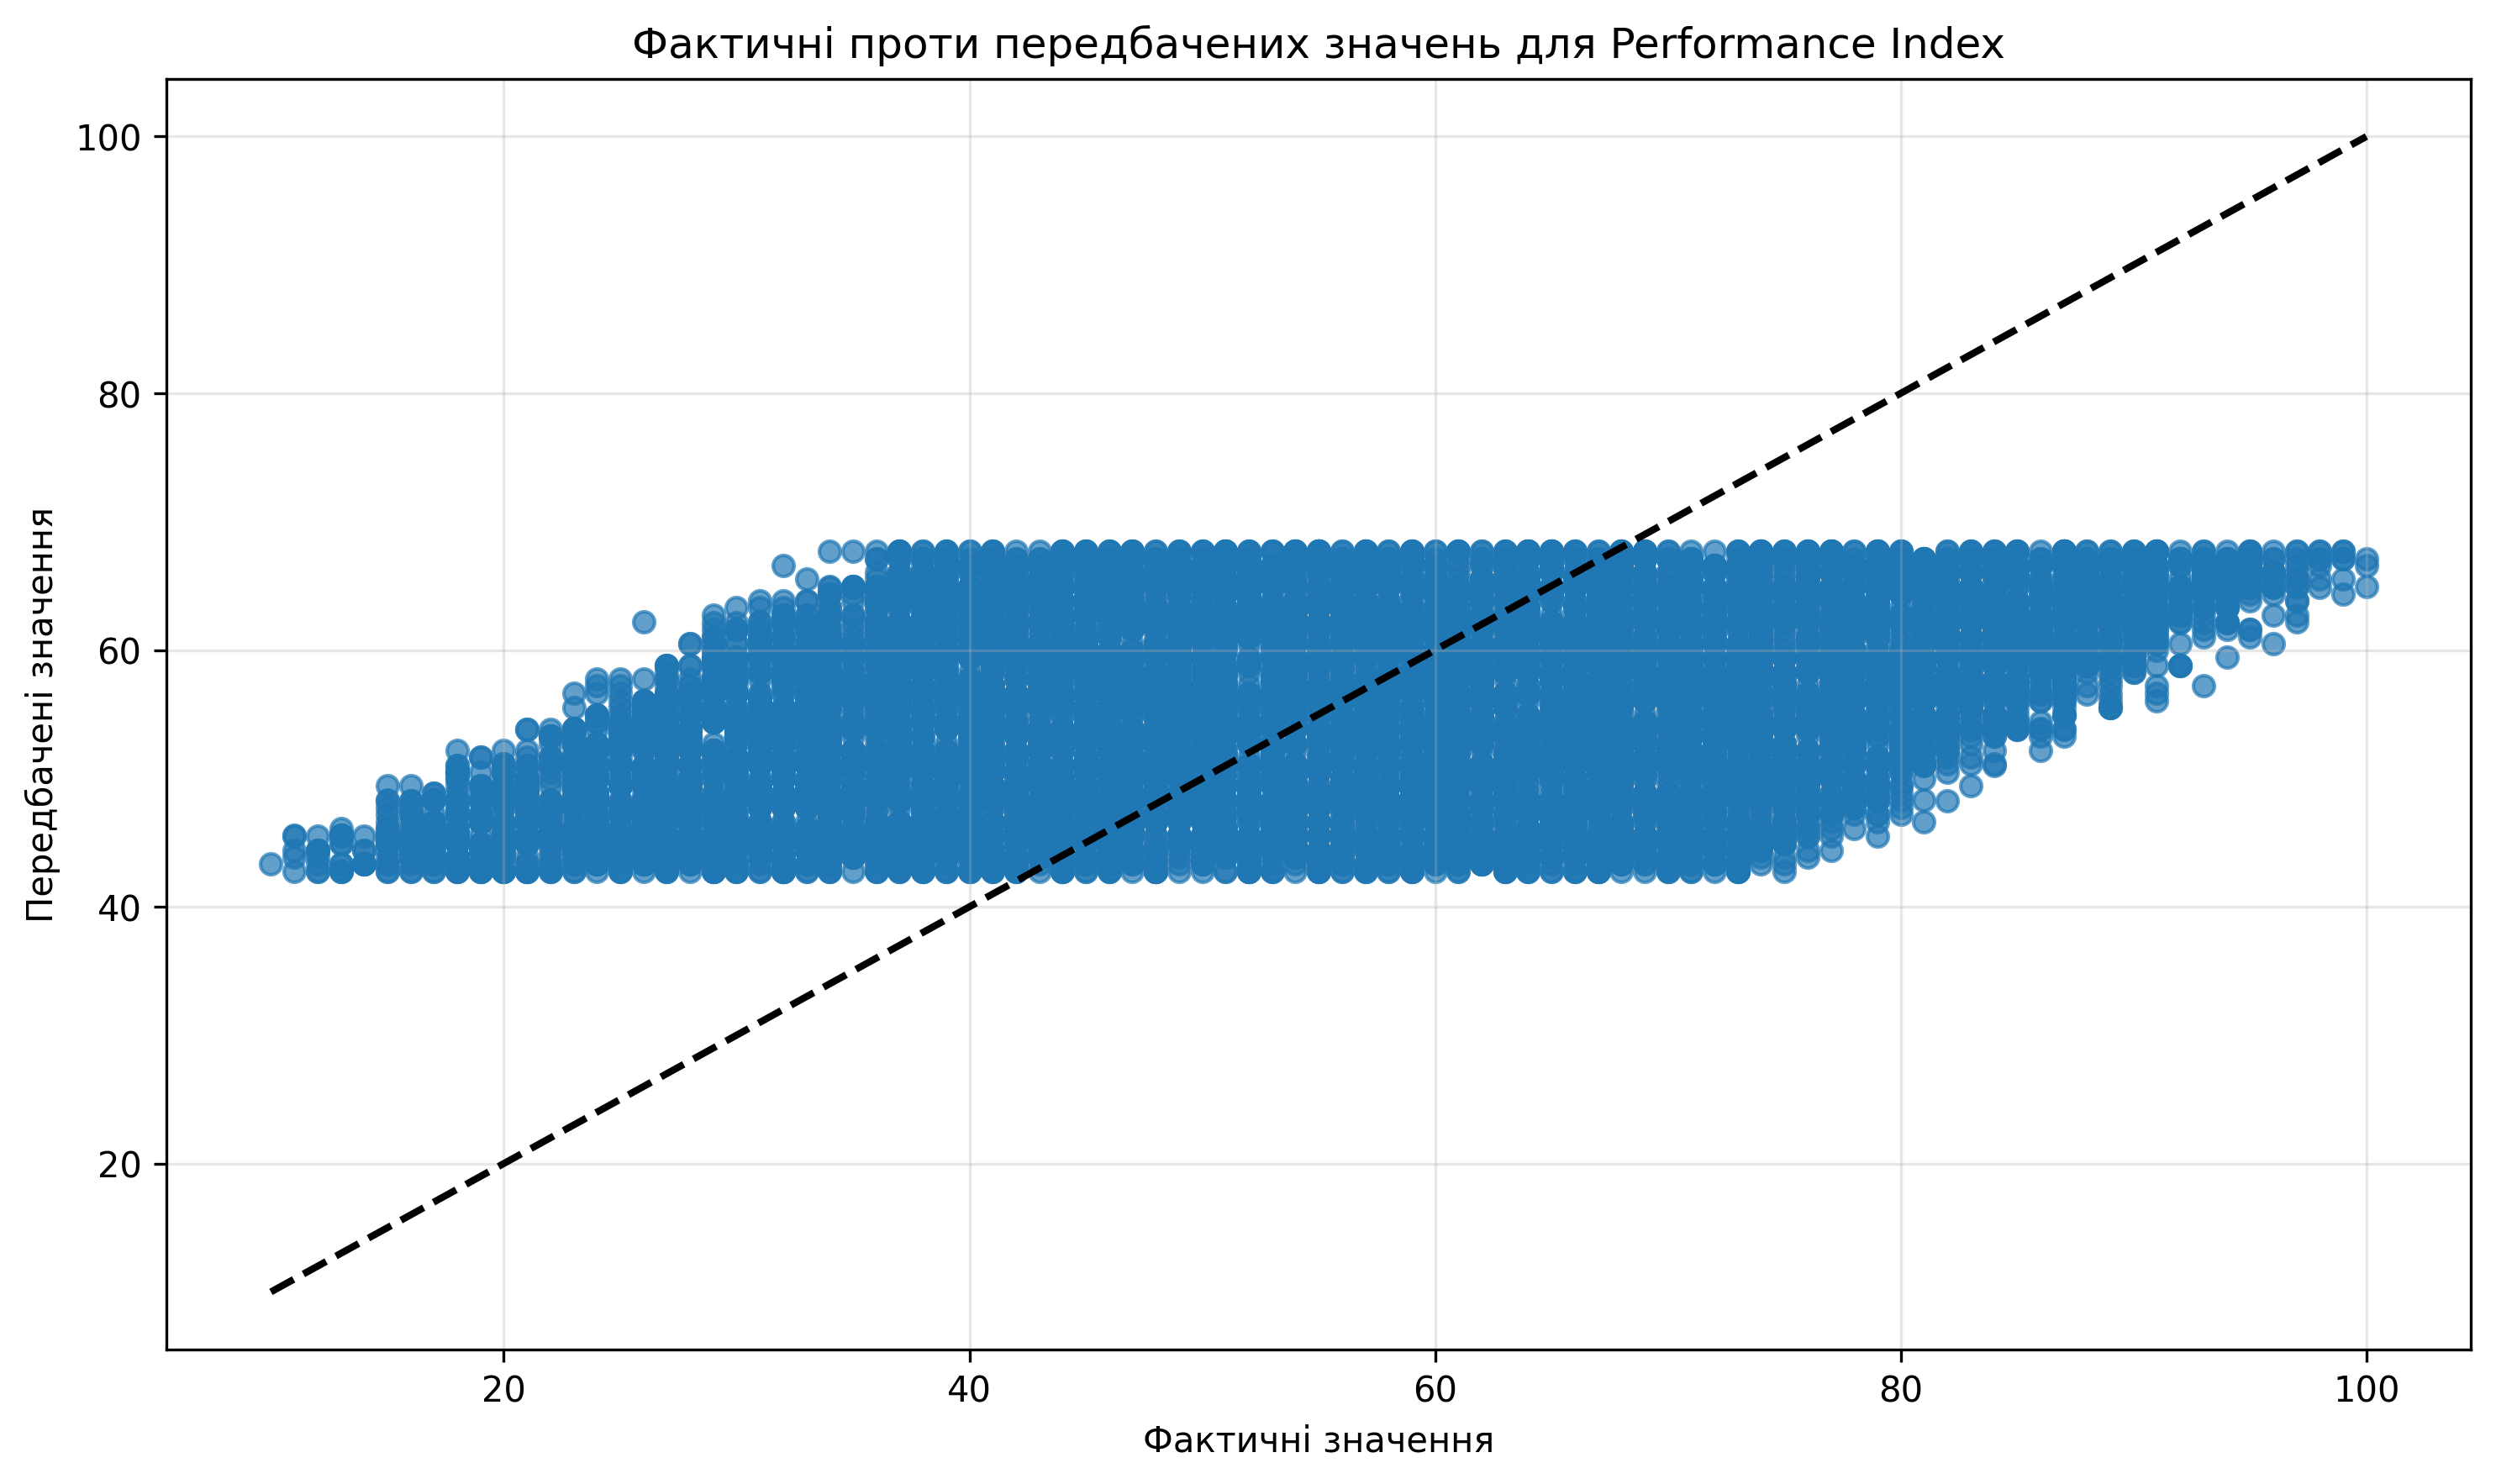
\includegraphics[width=0.8\textwidth]{actual_vs_predicted.png}
       \caption{Фактичні проти передбачених значень}
       \label{fig:фактичні_проти_передбачених_значень}
    \end{figure}

    \vspace{0.5cm}
    
    \begin{figure}[H]
       \centering
       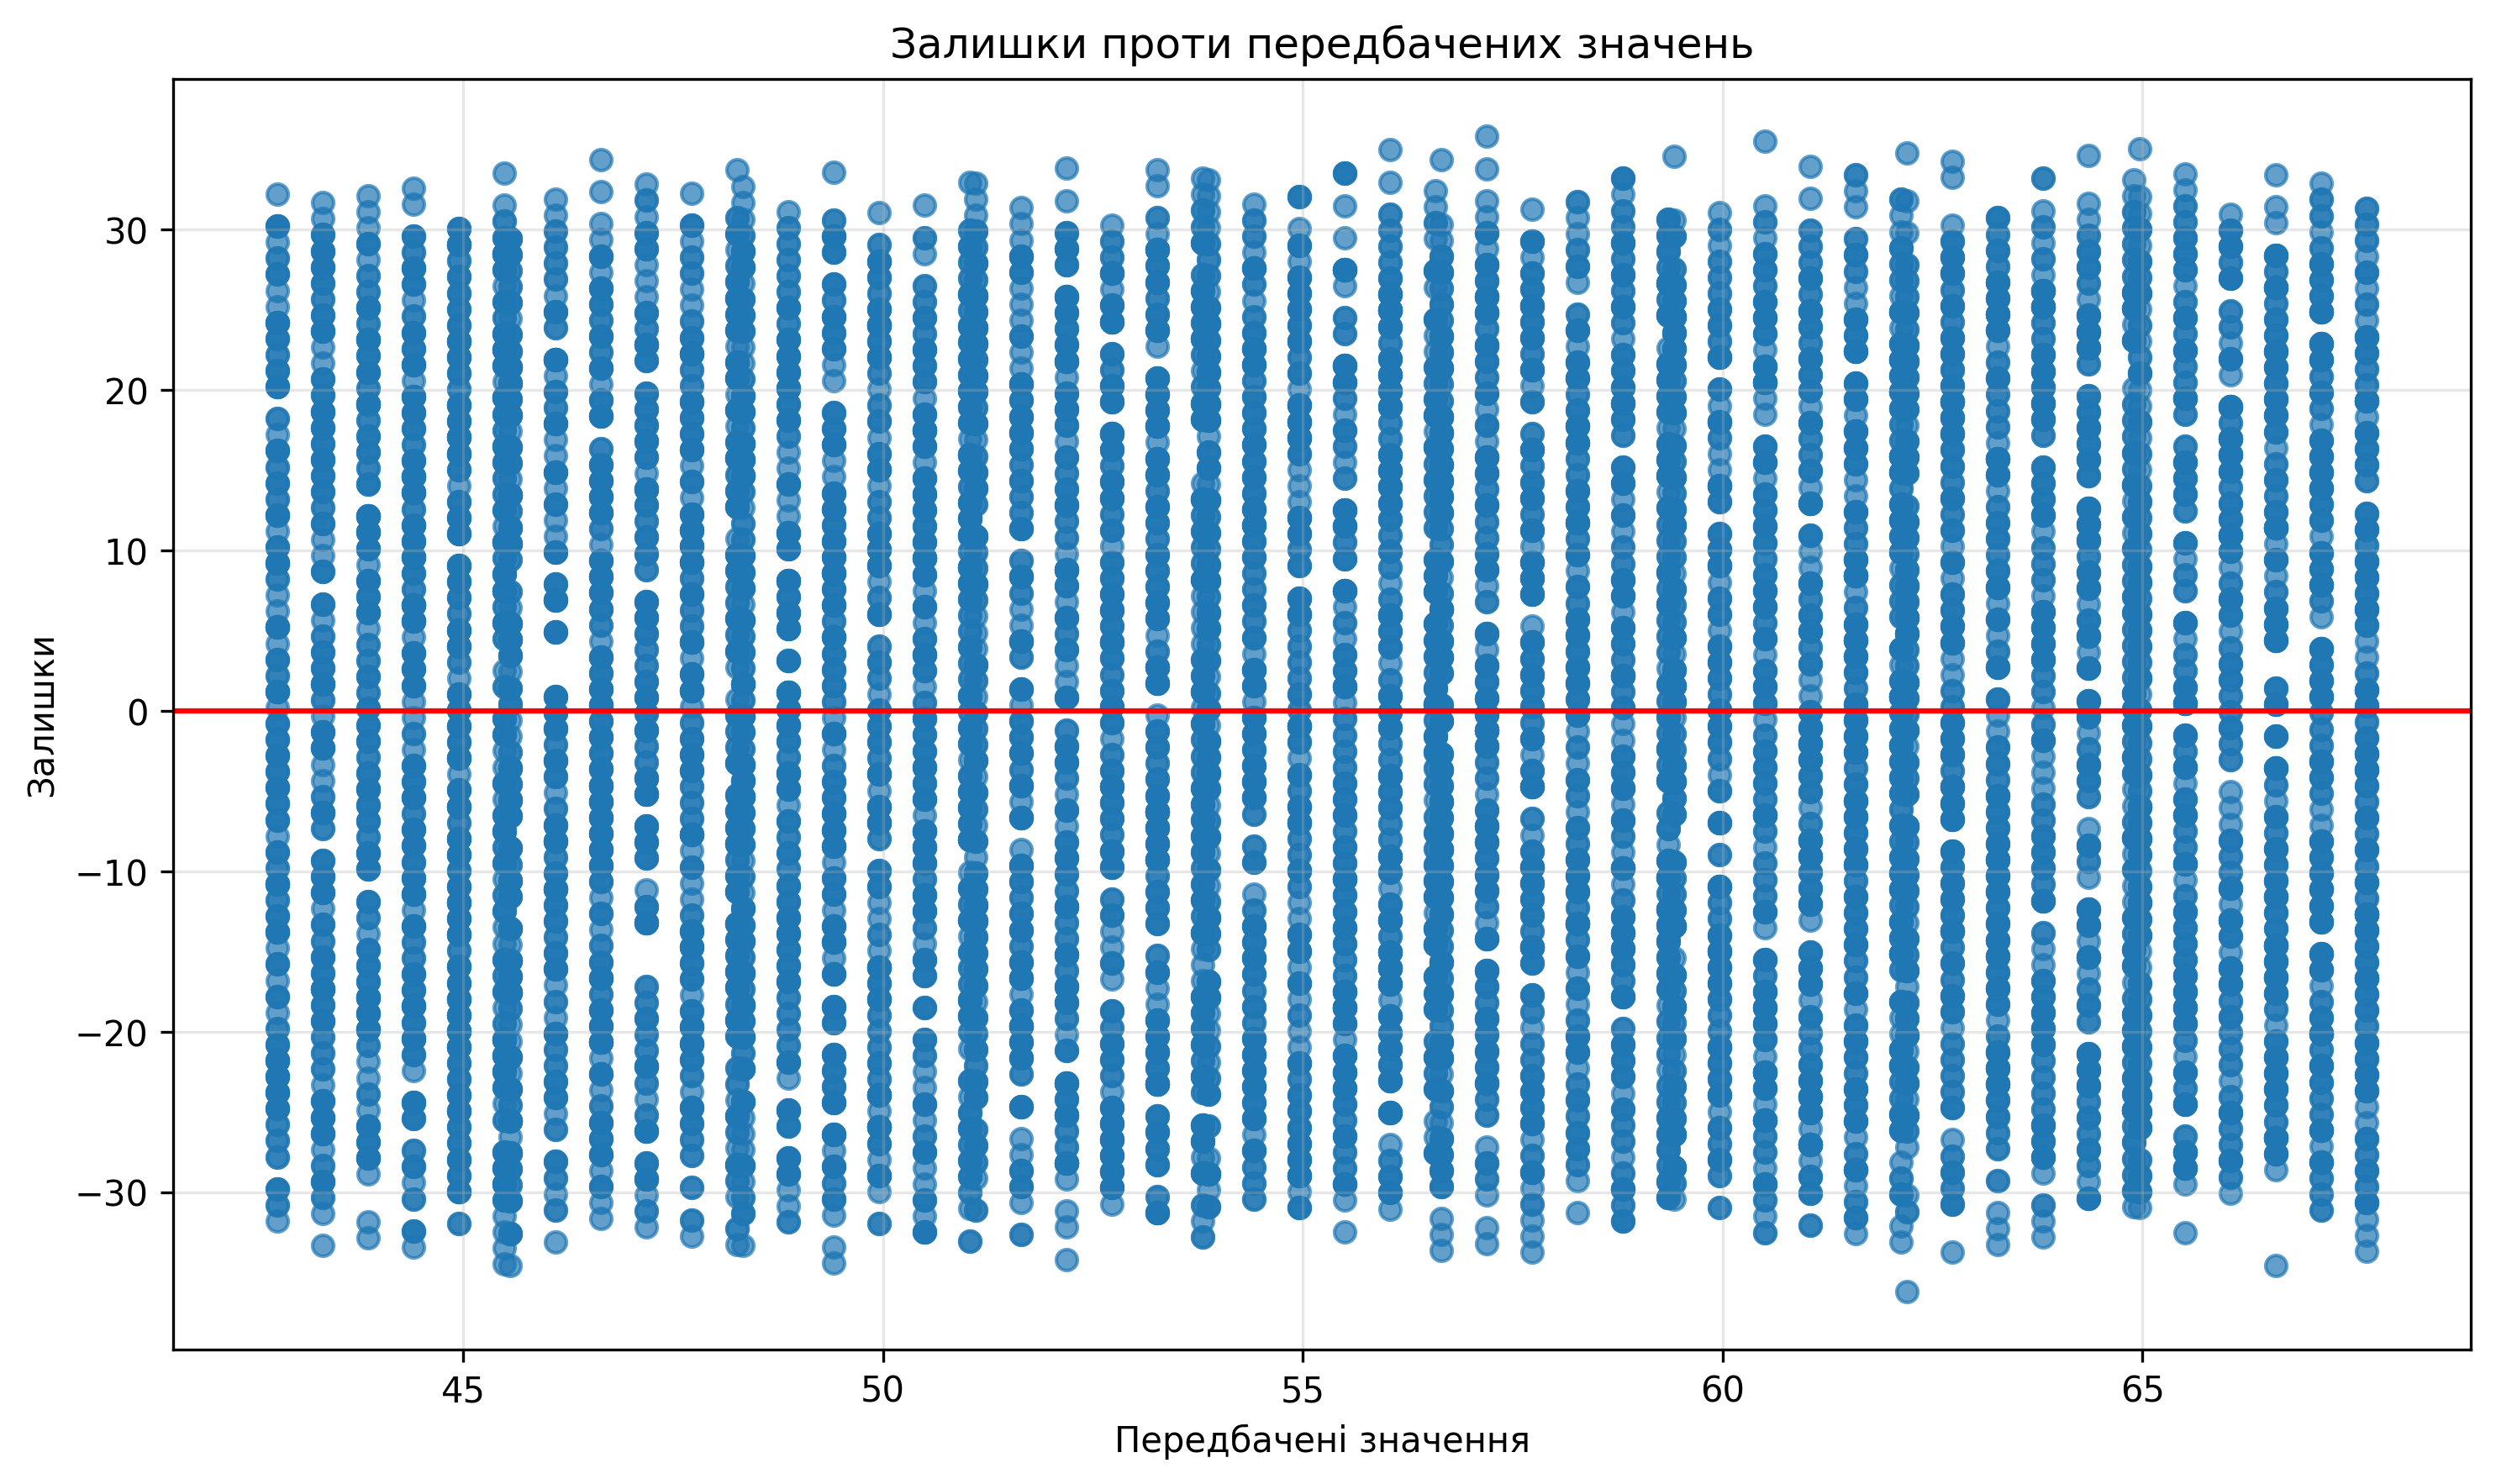
\includegraphics[width=0.8\textwidth]{residuals.png}
       \caption{Графік залишків}
       \label{fig:графік_залишків}
    \end{figure}

    \vspace{0.5cm}
    
    \begin{figure}[H]
       \centering
       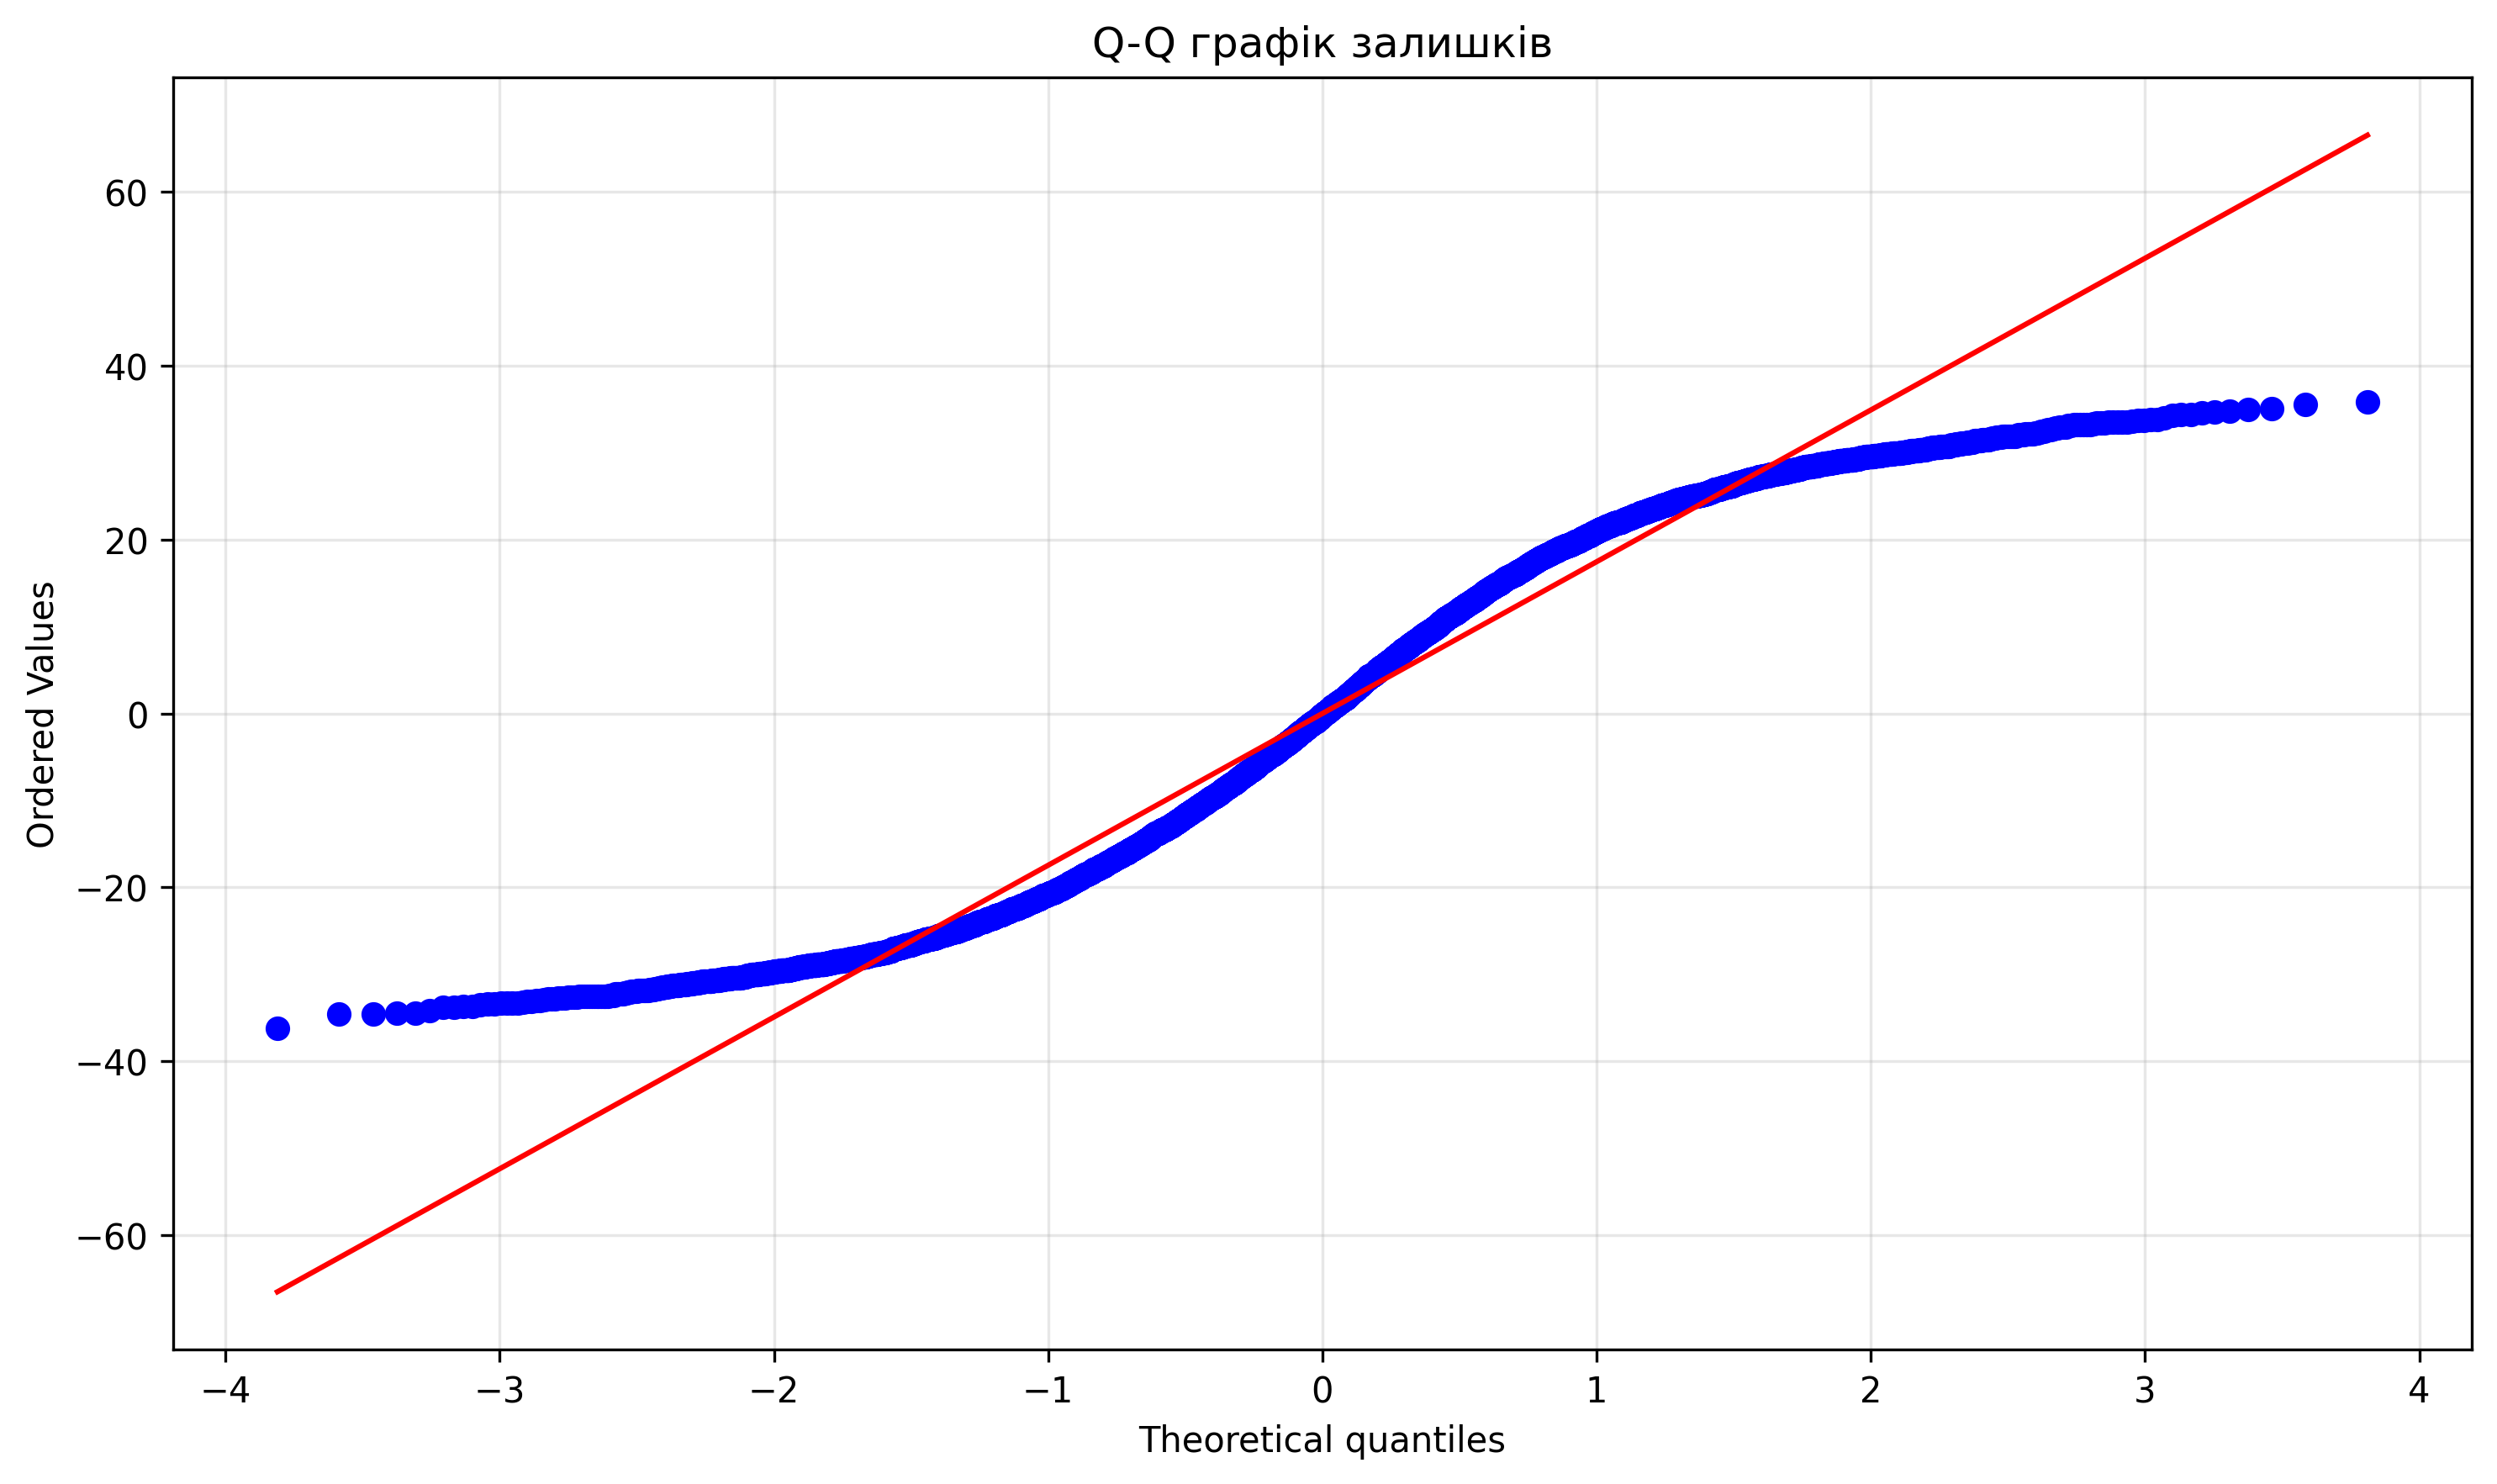
\includegraphics[width=0.8\textwidth]{qq_plot.png}
       \caption{Нормальний Q-Q графік залишків}
       \label{fig:нормальний_q-q_графік_залишків}
    \end{figure}

    \vspace{0.5cm}
    
    \begin{figure}[H]
       \centering
       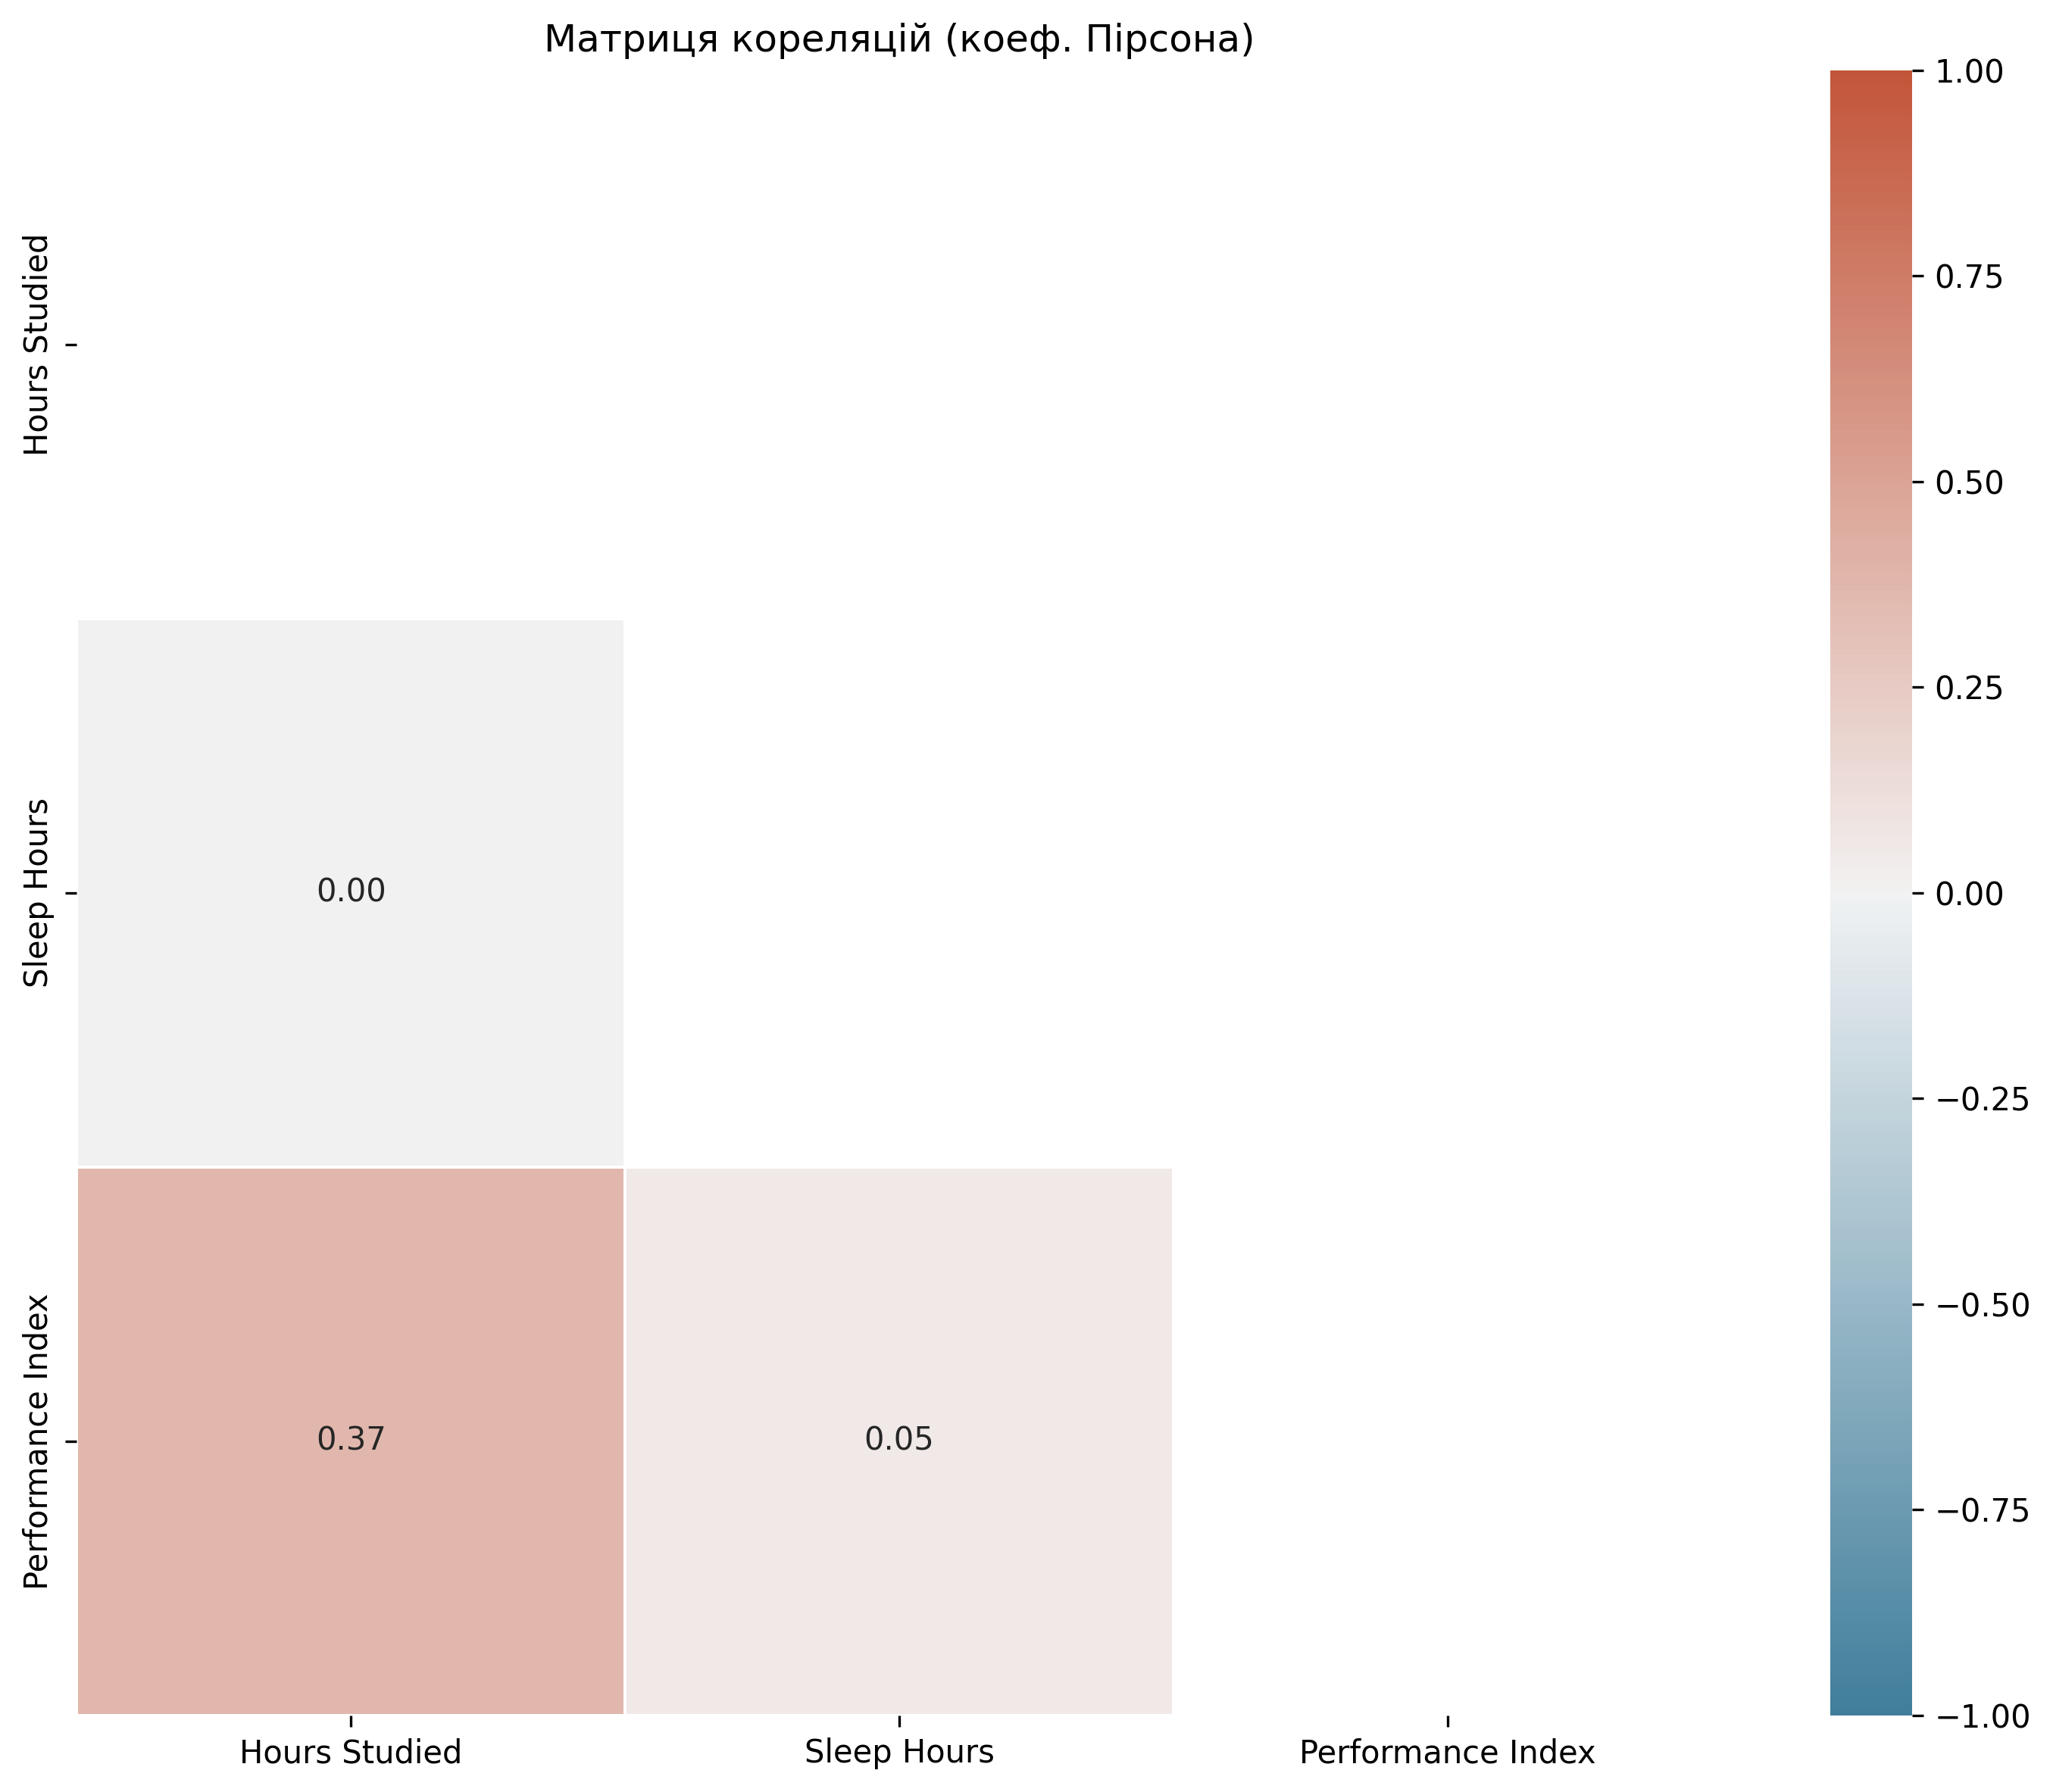
\includegraphics[width=0.8\textwidth]{correlation_heatmap.png}
       \caption{Теплова карта кореляцій (коеф. Пірсона)}
       \label{fig:теплова_карта_кореляцій_(коеф._пірсона)}
    \end{figure}

    \vspace{0.5cm}
    
    \begin{figure}[H]
       \centering
       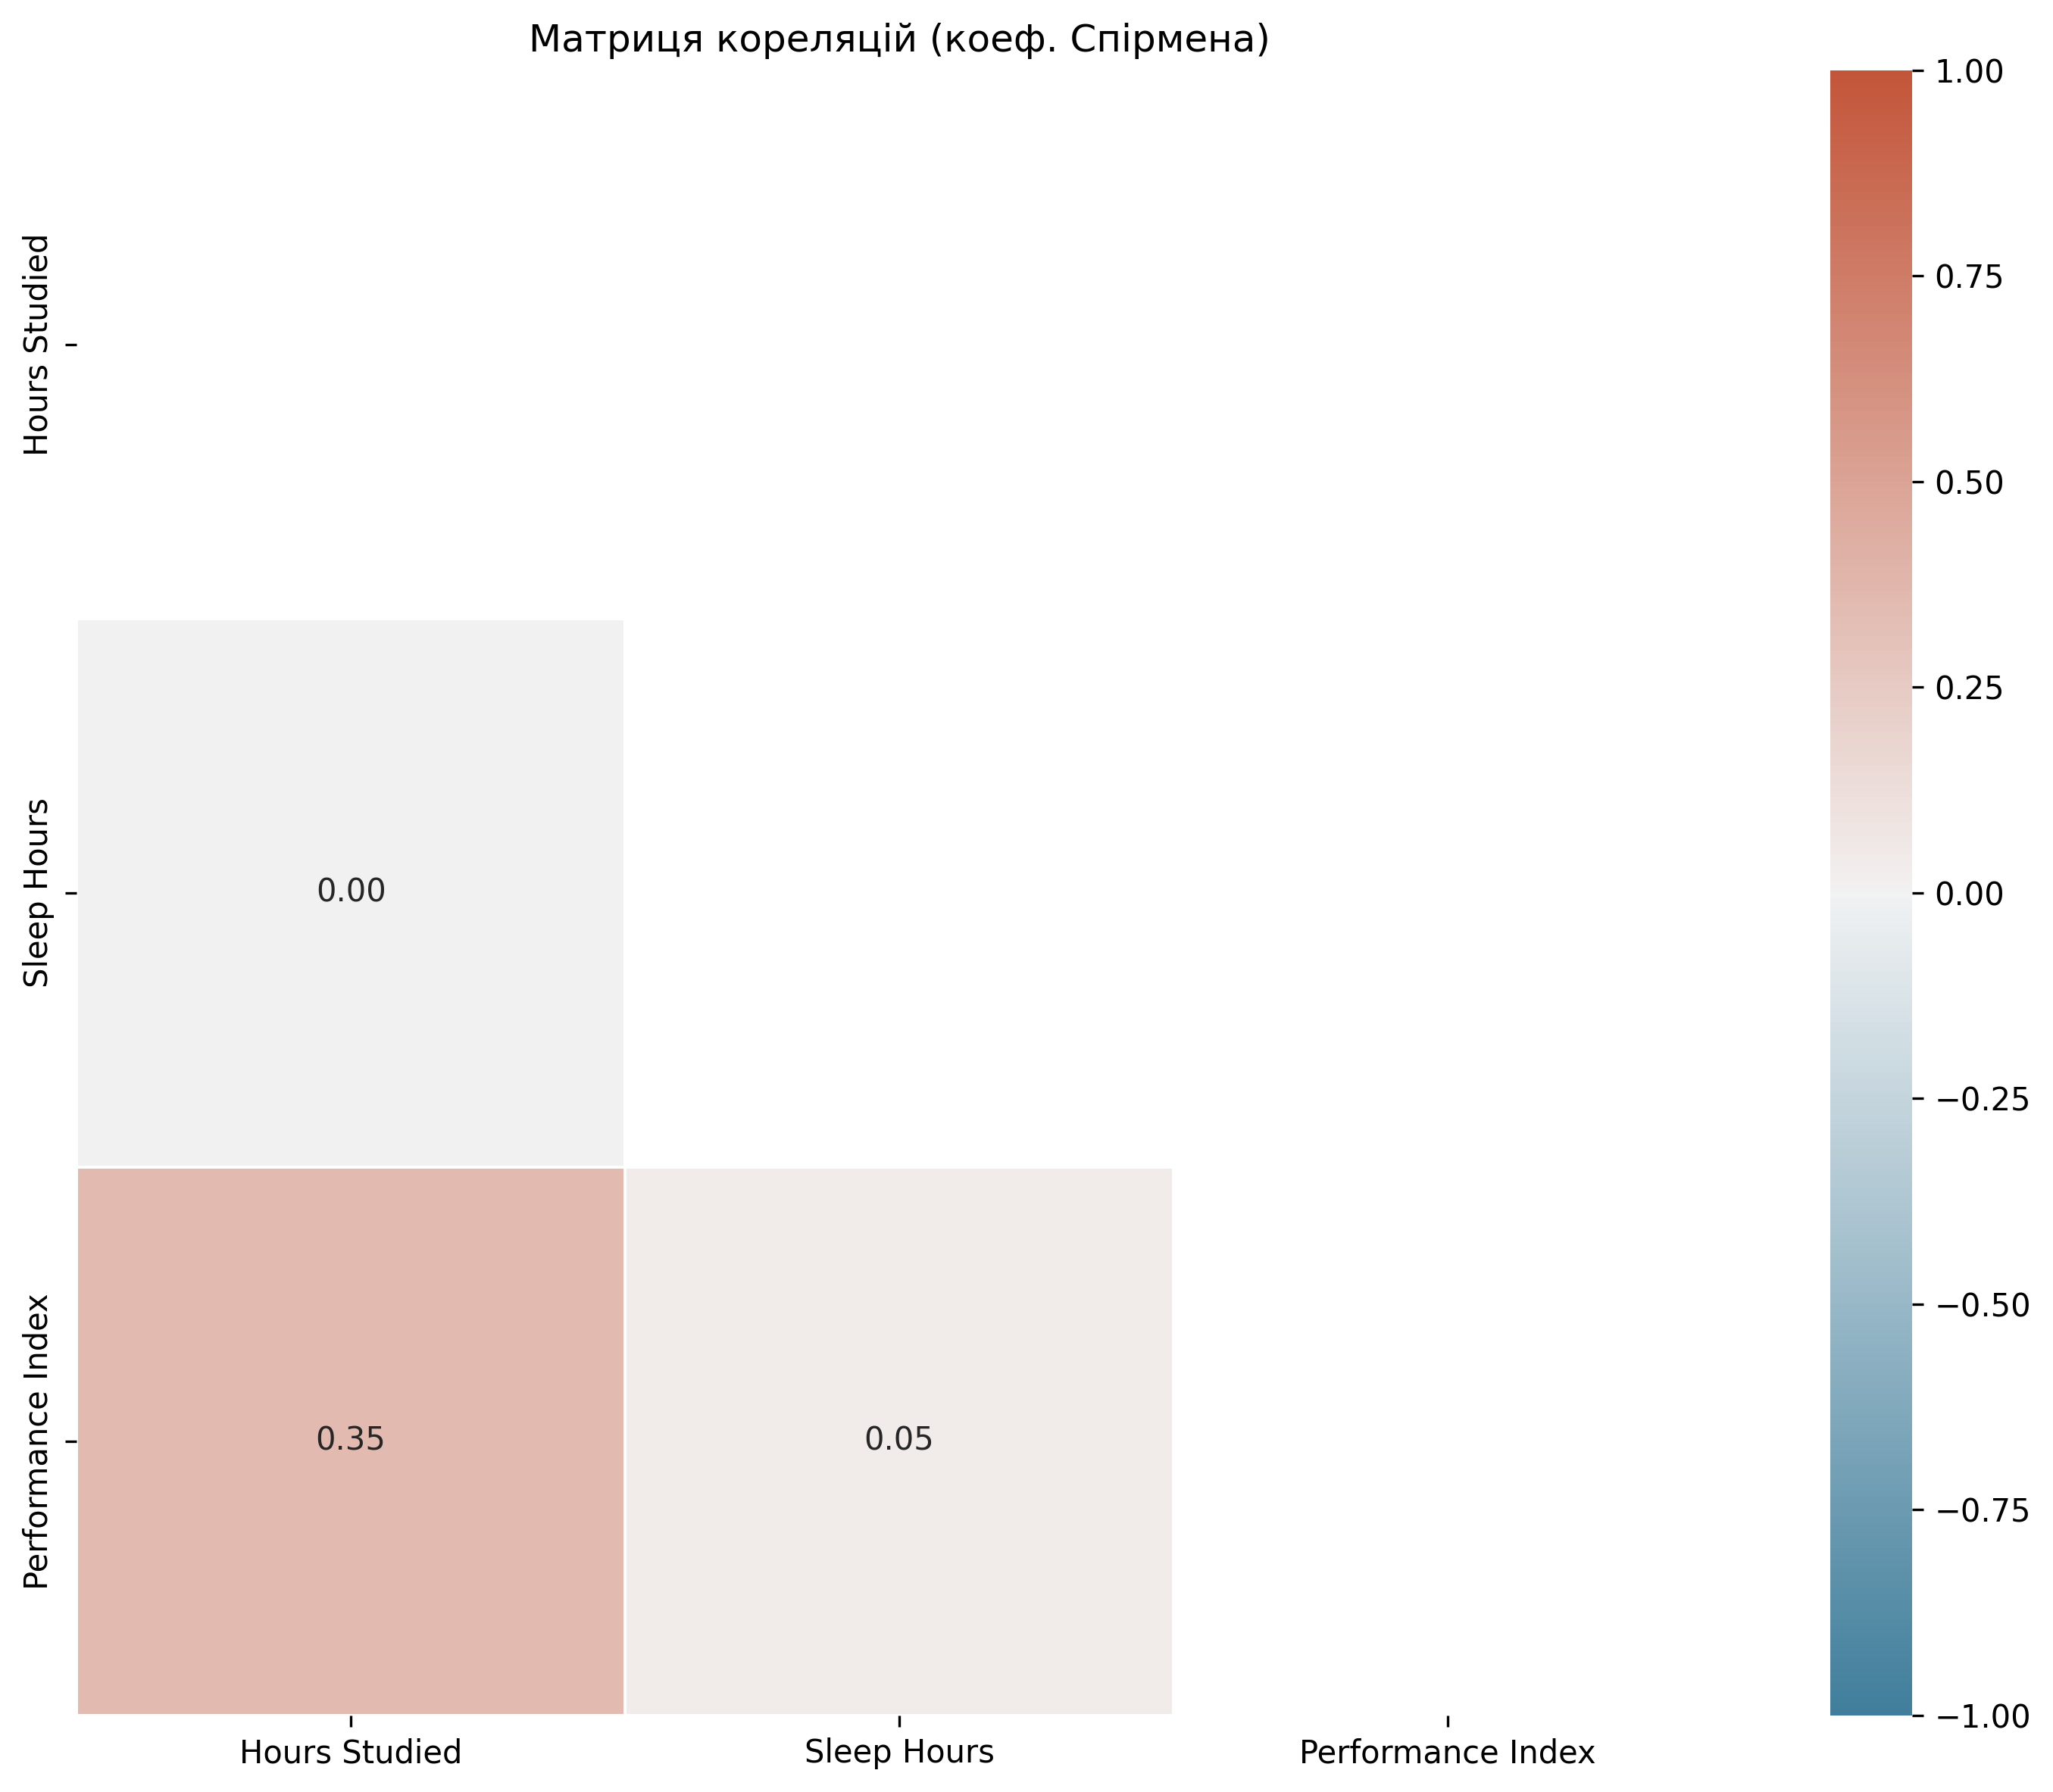
\includegraphics[width=0.8\textwidth]{correlation_heatmap_spearman.png}
       \caption{Теплова карта кореляцій (коеф. Спірмена)}
       \label{fig:теплова_карта_кореляцій_(коеф._спірмена)}
    \end{figure}

    \vspace{0.5cm}
    
    \begin{figure}[H]
       \centering
       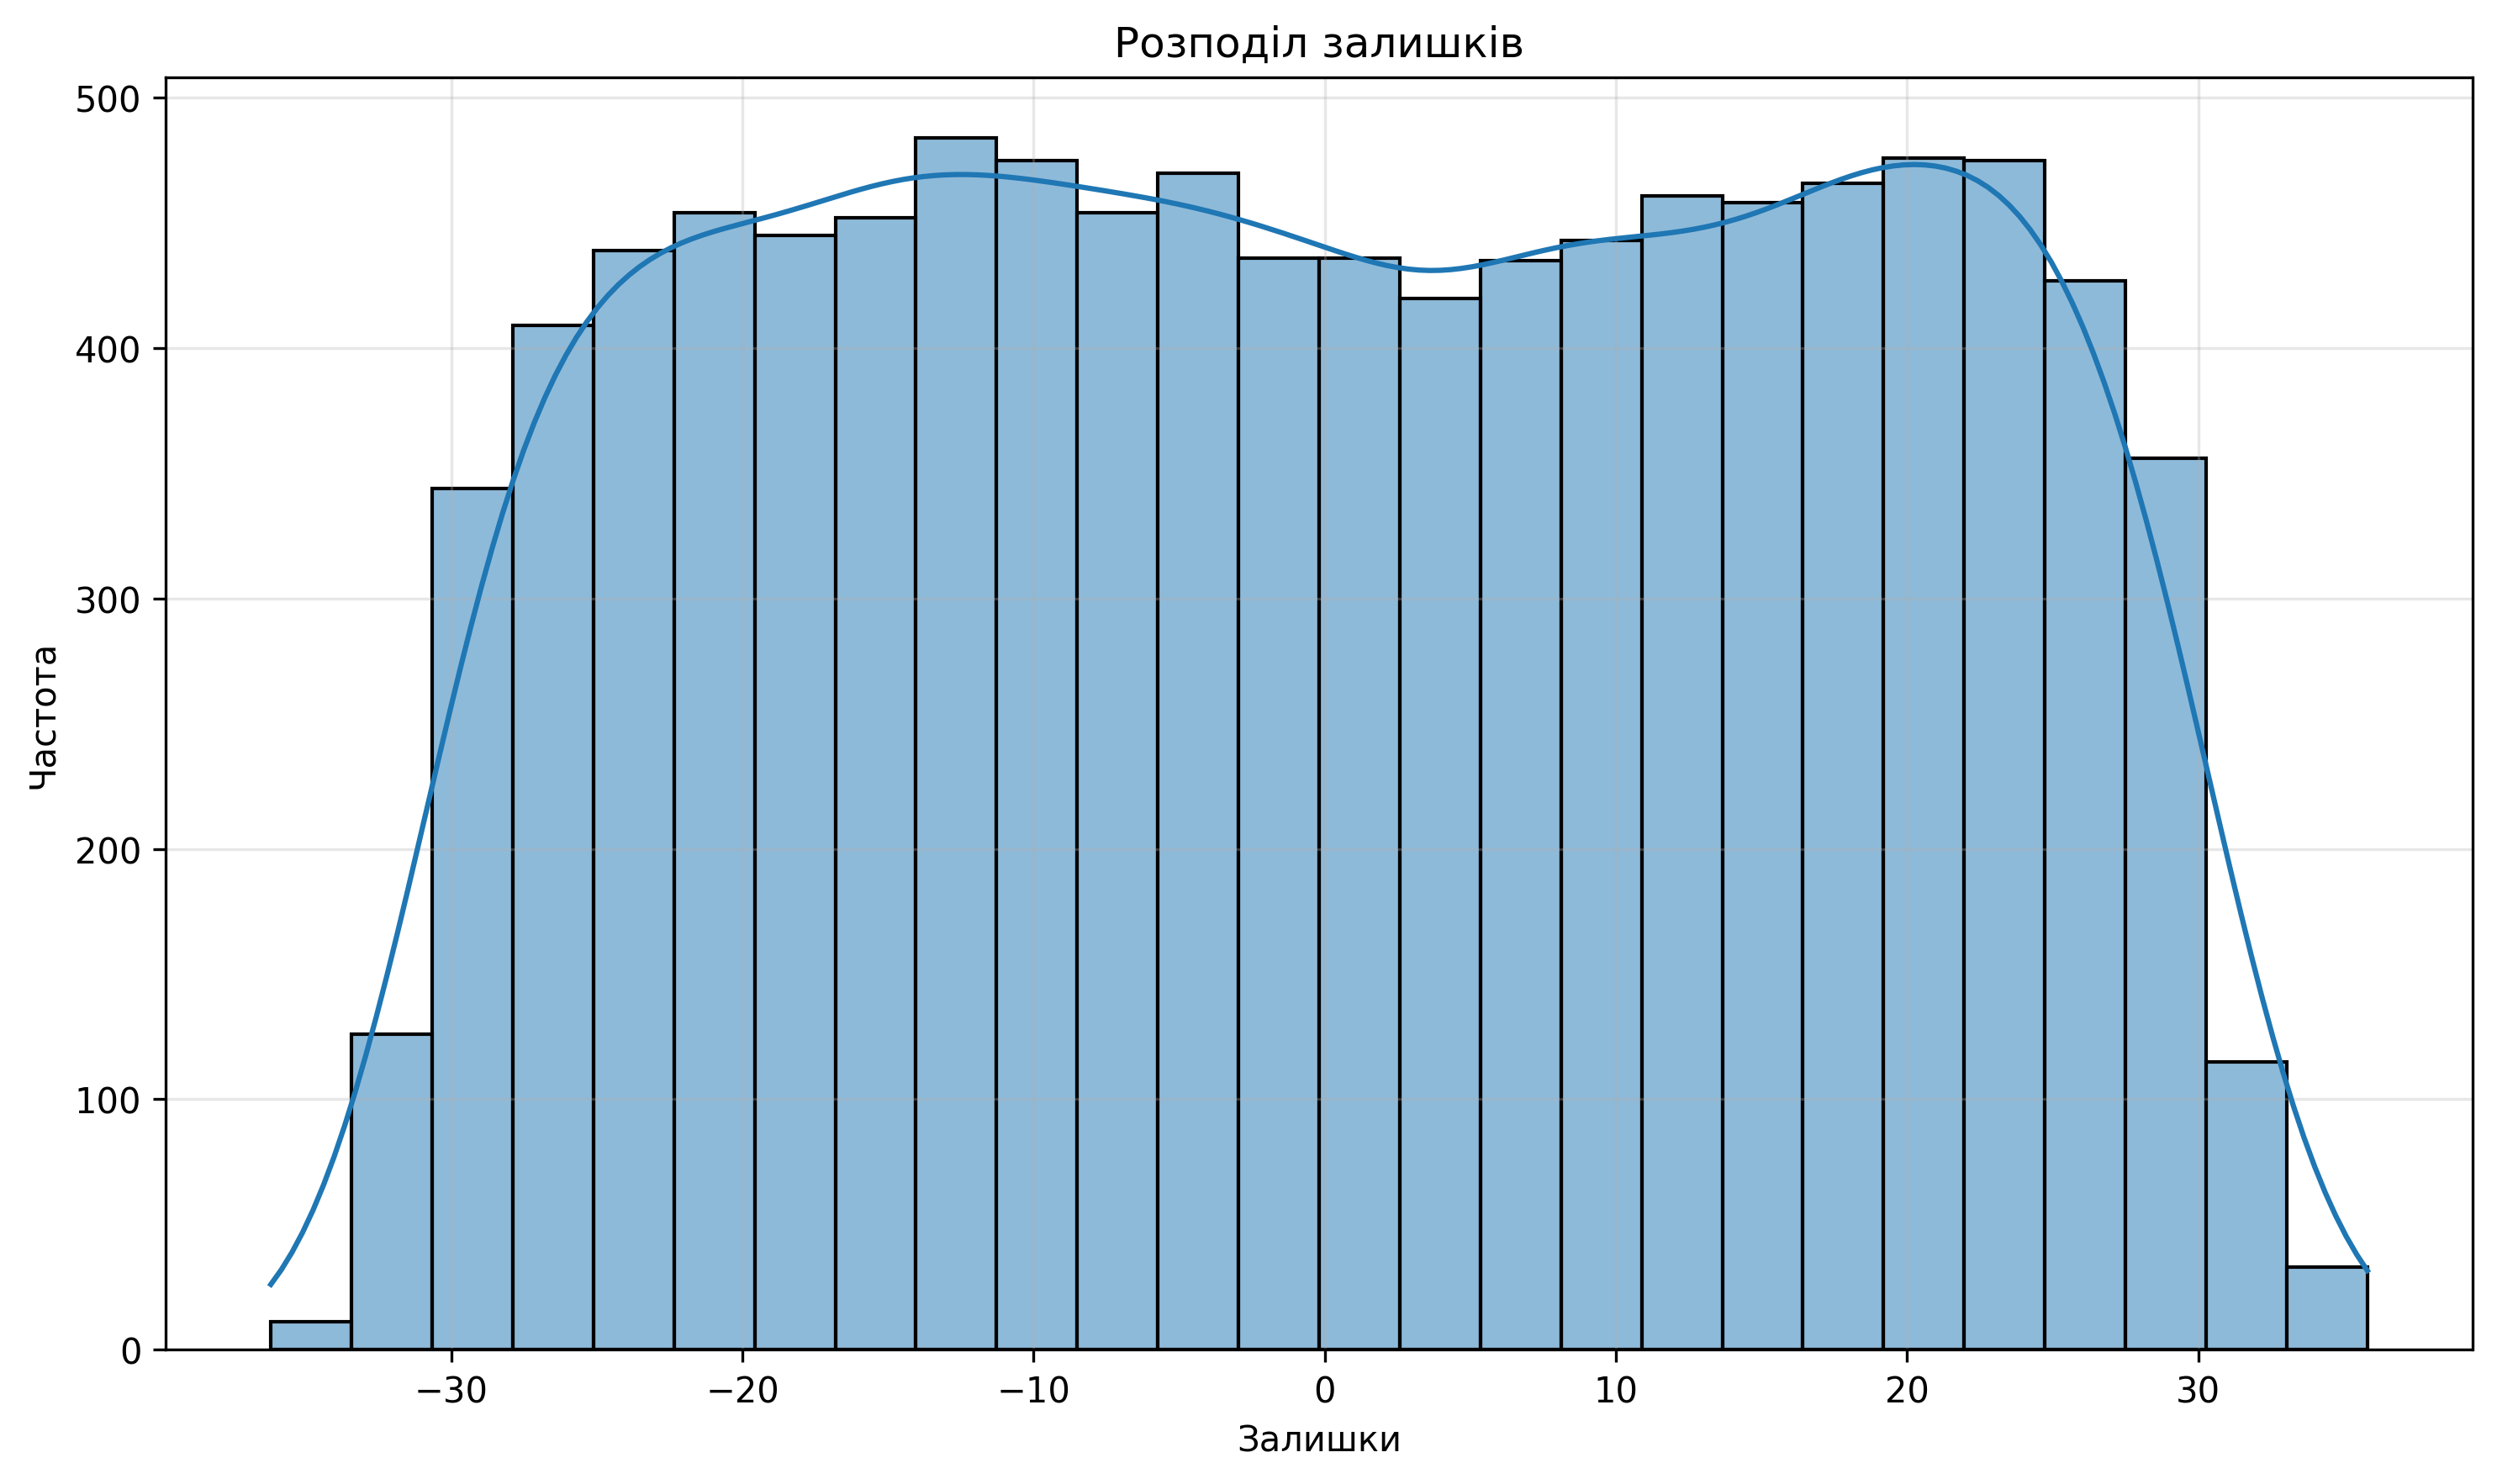
\includegraphics[width=0.8\textwidth]{residuals_hist.png}
       \caption{Гістограма залишків}
       \label{fig:гістограма_залишків}
    \end{figure}

    \vspace{0.5cm}
    

    \section{Інтерпретація результатів}

    Дана модель багатофакторної лінійної регресії показує залежність змінної \textbf{Performance Index} від змінних \textbf{Hours Studied}, \textbf{Sleep Hours}.

    Коефіцієнт детермінації $R^2$ дорівнює 0.1419, що означає, що 14.2\% варіації залежної змінної пояснюється включеними у модель незалежними змінними.

    Середньоквадратична похибка (MSE) становить 316.6960, що є мірою середнього квадратичного відхилення спостережуваних значень від передбачених.

    \vspace{0.5cm}

    \section{Висновки}

    Результати аналізу показують, що модель має низьку пояснювальну здатність.
    
    Найбільший вплив на залежну змінну мають фактори:
    \begin{itemize}
        \item \textbf{Hours Studied}: збільшує значення залежної змінної на 2.7726 одиниць при зміні на одну одиницю
    \item \textbf{Sleep Hours}: збільшує значення залежної змінної на 0.5397 одиниць при зміні на одну одиницю
\end{itemize}
    
    \end{document}
    